\documentclass[doktyp=barbeit]{TUBAFarbeiten}

\usepackage{selinput}% Auswahl der Dateikodierung (ansi,latin1,utf8,...)
	\SelectInputMappings{adieresis={ä},germandbls={ß},Euro={€}}% Zeichenzuordnung für selinput.sty
\usepackage[T1]{fontenc}% Einstellung Fontencoding

\usepackage{csquotes}% Einstellung zu Anführungszeichen; wird von biblatex.sty gefordert
\usepackage[backend=biber,sortlocale=de_DE_phonebook]{biblatex}% bessere Literaturverarbeitung
\addbibresource{tubafarbeiten-beispiel.bib}% welche Literaturdatenbank genutzt werden soll; Endung nicht vergessen!

%\usepackage{setspace}% Einstellungen Zeilenabstand
	%\onehalfspacing% Einstellungen Zeilenabstand

\setcounter{secnumdepth}{4}
% \setcounter{tocdepth}{4}

\TUBAFFakultaet{Fakultät für Mathematik und Informatik}
\TUBAFInstitut{Institut für Informatik}
\TUBAFLehrstuhl{Lehrstuhl für Betriebssysteme und Kommunikationstechnologien}

%\TUBAFZweitlogo{\includegraphics{thekla_logo.jpg}}

\TUBAFTitel[Entwicklung einer Sicherheitsinfrastruktur zur Bluetooth-Kommunikation zwischen Smartphone und Mikrocontroller]{Entwicklung einer Sicherheitsinfrastruktur zur Bluetooth-Kommunikation zwischen Smartphone und Mikrocontroller}
\TUBAFBetreuer{\,Prof.\,Dr. Konrad Froitzheim}
\TUBAFKorrektor{M.Sc. Jonas Treumer}%TODO Betreuer Lorenzo Neumann
\TUBAFAutor[M. Käsemodel]{Marian Käsemodel}
\TUBAFStudiengang{Angewandte Informatik}
\TUBAFVertiefung{Technik}
\TUBAFMatrikel{62\,412}
\TUBAFDatum[]{\today}%TODO

\begin{document}

\maketitle

\TUBAFErklaerungsseite


\KOMAoptions{
	listof=totoc	% Abbildungs- und Tabellenverzeichnis im Inhaltsverzeichnis
}

\tableofcontents
\newpage
\listoffigures
\listoftables

\newpage
\section{Einleitung}

	\subsection{Themenstellung}
		% TODO

	\subsection{Problemstellung}
		Ziel der Arbeit ist zunächst die Untersuchung der Schwachstellen innerhalb von \textit{Bluetooth Low Energy}. Dazu muss ein tieferes Verständnis für dessen Funktionsweise und die zur Verfügung gestellten Sicherheitsfunktionen gewonnen werden. Auf diesem Wissen aufbauend wird eine Infrastruktur entworfen, durch die ein Smartphone und ein Mikrocontroller mittels \textit{Bluetooth Low Energy} sicher miteinander kommunizieren können. Weder bei der Übertragung noch bei der Verarbeitung innerhalb des Systems soll eine außenstehende Instanz auf die übertragenen Nachrichten zugreifen können. Demnach ist eine Lösung für die Probleme der Authentizität, Datenintegrität und Vertraulichkeit erforderlich. Im Idealfall ist die Infrastruktur nicht nur auf die Geräte Smartphone und Mikrocontroller beschränkt, sondern wäre für jede Art von Bluetooth-Gerät denkbar.
\\\\
Desweiteren ist es Ziel der Arbeit, mithilfe dieser Infrastruktur eine Implementierung umzusetzen, die sich auf das Projekt \textit{SteigtUM} bezieht. Da bei dem vorgestellten Verleihdienst sensible Daten zwischen Smartphone und Fahrzeug ausgetauscht werden, wird die Infrastruktur als Grundlage für die sichere Kommunikation genutzt. Dennoch sind weitere Lösungen gefordert. Nur der Nutzer darf Zugriff auf die Funktionen des ausgeliehenen Fahrzeugs erlangen. Demnach muss zu Beginn eines Ausleihprozesses sichergestellt werden, dass der Nutzer berechtigt ist, das Fahrzeug auszuleihen. Verlässt er das Fahrzeug und möchte es nach einer bestimmten Zeit wieder nutzen, soll kein anderer in der Lage sein, das Fahrzeug in der Zwischenzeit zu entsperren und zu entwenden.

\newpage
\section{Grundlagen zu Bluetooth Low Energy}

	\subsection{Überblick}
		Bluetooth ist ein Industriestandard für die Übertragung von Daten per Funk, dessen Intention die Reduzierung von Kabelverbindungen an mobilen sowie stationären Geräten ist. Wichtige Eigenschaften der Technologie sind vor allem ein niedriger Energieverbrauch und günstig herstellbare Hardware. Seit 1998 wird Bluetooth von der \textit{Bluetooth Special Interest Group} (SIG) entwickelt und ist seit 2002 von der \textit{Organisation Institute of Electrical and Electronics Engineers} (IEEE) standardisiert \cite{IEEE}.
% QUELLE https://standards.ieee.org/standard/802_15_1-2002.html)
\\\\
Es agiert im lizenzfreien ISM-Band (Industrial, Scientific and Medical Band) von 2,4 GHz. 
% TODOOPT QUELLE
% BR/EDR: BT Specification 4.0 PDF S. 124, 1.1 Overview of BR/EDR Operation, 1. Absatz
% LE: BT Specifiaction 4.0 PDF S. 126, 1.2 OVERVIEW OF BLUETOOTH LOW ENERGY OPERATION, 1. Absatz
Zur Reichweite kann keine genaue Aussage getroffen werden, da sie von vielen Parametern wie beispielsweise der Sendeleistung und Einflüssen aus der Umwelt abhängt. Um trotzdem einen Eindruck zu gewinnen, kann für bestimmte Bedingungen und Konfigurationen die maximale Reichweite mithilfe eines Tools \cite{BtRangeTool} der SIG ermittelt werden. Dabei variieren die Ergebnisse von ca. einem Meter bis hin zu mehr als 1000 Metern.
% QUELLE https://www.bluetooth.com/learn-about-bluetooth/key-attributes/range/
\\\\
Grundlegend wird Bluetooth seit der Version 4.0 von 2010 in die zwei Systeme \textit{Basic Rate} (BR) und \textit{Low Energy} (LE) unterteilt, wobei LE darauf ausgelegt ist, weniger Energie als BR zu benötigen. Die neueste Bluetooth"=Version ist die Version 5.2, die wie jede Version abwärtskompatibel ist. Jedoch sind beide Systeme (BR und LE) bezüglich der Kommunikation miteinander inkompatibel: implementiert ein Gerät nur das BR"=System, kann es keine Daten mit einem Gerät austauschen, das nur das LE"=System unterstützt. Demnach ist für LE die Abwärtskompatibilität nur bis zur Version 4.0 gegeben. Desweiteren ist es möglich, dass ein Gerät über beide Systeme verfügt und so die meisten Nutzungsfälle abdeckt. Das BR"=System kann mit den Erweiterungen \textit{Enhanced Data Rate} (EDR) und \textit{Alternate Media Access Control and Physical Layer} (AMP) genutzt werden, um eine höhere Datenrate zu erzielen. Die einzelnen Systeme und Erweiterungen können entsprechend ihrer Bluetooth-Version die in Tabelle \ref{tab: maximale Bitraten BT} dargestellten Datenraten erreichen.
\begin{table}[H]
    \begin{tabular}[h]{|l|l|l|}
    \hline
    \textbf{System/Erweiterung} & \textbf{max. Bitrate (Version 4.0)} & \textbf{max. Bitrate (Version 5.2)} \\
    \hline
    BR          & 1 Mbit/s \cite{BtSpec4.0_124}               & 1 Mbit/s \cite{BtSpec5.2_188}           \\
    \hline
    BR/EDR      & 2 Mbit/s bis 3 Mb/s \cite{BtSpec4.0_124}    & 2 Mbit/s bis 3Mb/s \cite{BtSpec5.2_188} \\
    \hline
    802.11 AMP  & 24 Mbit/s \cite{BtSpec4.0_123}              & 52 Mbit/s \cite{BtSpec5.2_187}          \\
    \hline
    LE          & 1 Mbit/s \cite{BtSpec4.0_126}               & 2 Mbit/s \cite{BtSpec5.2_190}           \\
    \hline
    % QUELLE
    % BT Specification 4.0 PDF S. 124, 1.1 Overview of BR/EDR Operation, 1. Absatz
    %                          S. 126, 1.2 OVERVIEW OF BLUETOOTH LOW ENERGY OPERATION, 1. Absatz
    % BT Specification 5.2 PDF S. 188 1.1 Overview of BR/EDR Operation, 1. Absatz
    %                          S. 190, 1.2 OVERVIEW OF BLUETOOTH LOW ENERGY OPERATION, 1. Absatz
    \end{tabular}
    \caption[Maximale Bitraten der Bluetooth-Systeme]{Maximale Bitraten der Bluetooth-Systeme}
    \label{tab: maximale Bitraten BT}
\end{table}
\textit{Da Bluetooth Low Energy (BLE) ein zentraler Bestandteil dieser Arbeit ist, bezieht sich der Autor von nun an nur darauf und nicht mehr auf Bluetooth im Allgemeinen. D.h., dass Bluetooth Classic, welches BR/EDR und AMP beschreibt, nur noch behandelt wird, wenn das BR"=System oder eine seiner Erweiterungen explizit erwähnt werden.}
\\\\
Die Architektur eines Bluetooth"=Systems unterteilt sich in einen Host und in einen oder mehrere Controller. Ein Host ist eine logische Entität, definiert als alle Schichten unterhalb der nicht zu Bluetooth gehörigen Profile (Protokolle) und oberhalb des Host"=Controller"=Interface (HCI). Ein Controller ist eine logische Entität, definiert als alle Schichten bzw. Funktionsblöcke unterhalb des HCI. Der Aufbau setzt sich immer aus genau einem primären Controller und optional aus sekundären Controllern zusammen. Dabei kann die Rolle des primären Controllers entweder durch einen BR/EDR"=Controller, einen LE"=Controller oder durch eine Kombination aus BR/EDR- und LE"=Controller eingenommen werden, während die Rolle eines sekundären Controllers nur durch einen AMP"=Controller besetzt werden kann. In Abb. \ref{fig: kombinationen aus host und controller} sind einige Varianten skizziert. 
% TODOOPT QUELLE BT Specification 4.0, PDF S.123 f.
\begin{figure}[H]
    \centering
    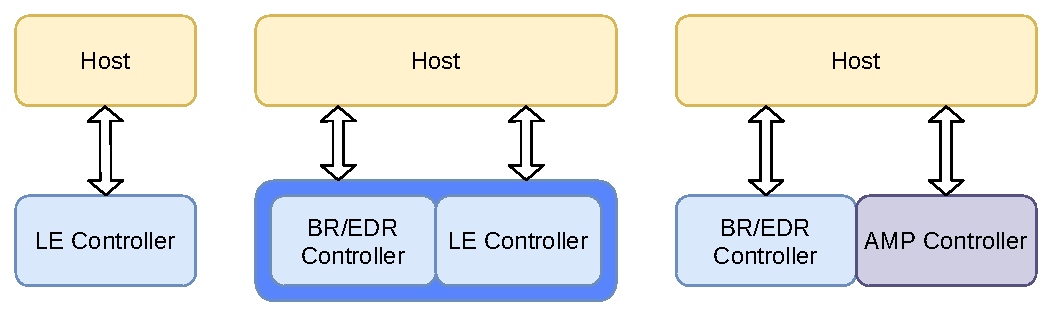
\includegraphics[width=0.9\linewidth]{graphics/kombination_host_controller.pdf}
    \caption[Kombinationen aus Host und Controller]{Kombinationen aus Host und Controller; in Anlehnung an \cite{BtSpec4.0_fig_124}}
    \label{fig: kombinationen aus host und controller}
\end{figure}
% QUELLE BILD BT Sepcification 4.0, PDF S. 124
Zur Veranschaulichung der Architektur bezüglich eines LE"=Systems ist in der Abb. \ref{fig: host controller architektur} die Zusammensetzung aus Host und Controller mit deren Schichten bzw. Protokollen festgehalten, die in den Sektionen \ref{sec: le controller} und \ref{sec: le host} thematisiert werden. Über dem Host befindet sich die Anwendungsschicht.
\begin{figure}[H]
    \centering
    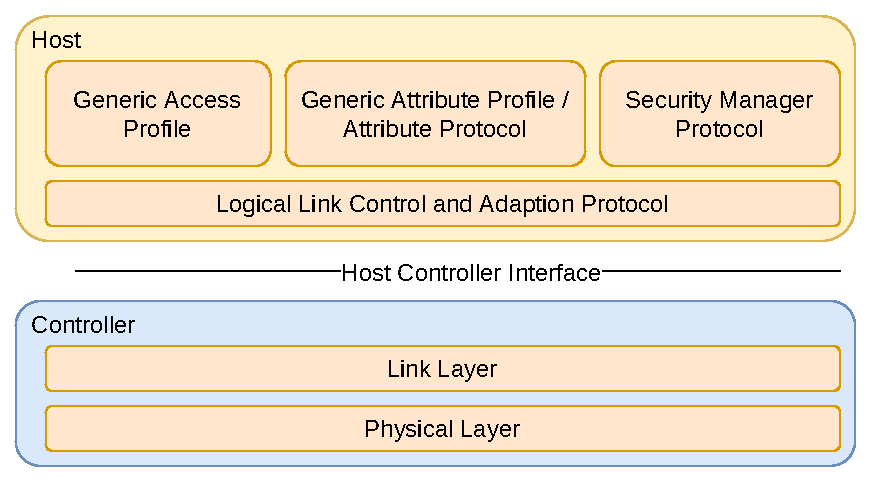
\includegraphics[width=0.7\textwidth]{graphics/host_controller_hci.pdf}
    \caption[BLE-Architektur von Host und Controller]{BLE-Architektur von Host und Controller; in Anlehnung an \cite{BtSpec4.0_fig_137}}
    \label{fig: host controller architektur}
\end{figure}

	\subsection{Topologie}
		Die Topologie der Infrastruktur beschränkt sich auf das Minimum an Kommunikationsparteien und ist unabhängig von der Anwendung.\\

% TODO BILD topologie infratruktur mikrocontroller, smartphone, CA

Dem Thema zufolge sollen ein Mikrocontroller und ein Smartphone sicher Daten austauschen. Um dies zu bewerkstelligen, wird über den Transport der Daten durch Bluetooth Low Energy (BLE) das Verschlüsselungsprotokoll TLS verwendet (siehe Sektion X). 
% TODO SEKTION VERWEIS Infrakstruktur->Sicherheit
Dementsprechend ist, wie in Abbildung X zu sehen
% TODO BILD VERWEIS topologie infrastruktur mikrocontroller, smartphone, CA
, neben dem Mikrocontroller und dem Smartphone eine Zertifizierungsstelle notwendig. In welcher Form diese auftritt ist von der Anwendung abhängig.

Für einen seriösen Anwendungsfall sollte die Zertifizierungsstelle evtl. in Form eines Servers existieren, der dem Mikrocontroller und Smartphone in regelmäßigen Abständen (z.B. jährlich) jeweils ein Zertifikat ausstellt. Mit diesen Zertifikaten und der Kenntnis über das Root-Zertifikat können Mikrocontroller und Smartphone sich gegenseitig authentifizieren und somit die Grundlage für eine sichere Kommunikation bilden.

Beispielsweise könnte es für einen privaten Anwendungsfall ausreichend sein, die Zertifizierungsstelle nicht als dauerhaft betriebenen Server darzustellen, sondern lediglich ein Root-Zertifikat zu erstellen und mit diesem dem Mikrocontroller und Smartphone jeweils ein digitales Zertifikat auszustellen.

Die Rolle der Partei, die die Zertifikate für Mikrocontroller und Smartphone austellt muss nicht zwingend eine Zertifizierungsstelle sein, sondern könnte auch eine Entität sein, der von einer Zertifizierungsstelle ein Zwischenzertifikat ausgestellt wurde.

	\subsection{Controller}
		Wie in Abbildung X
% TODO BILD VERWEIS letztes Bild aus überblick
zu sehen ist, umfasst der Controller die Schichten Physical Layer (PHY) und Link Layer (LL, auch Logical Layer genannt). Der Phyical Layer unterteilt sich weiter in die Physical Channels und die Phyical Links, während der Link Layer sich in Logical Transports und Logical Links aufteilt. In den Schichten bzw. ihren Untergliederungen wird definiert, wie Anwenderdaten, Advertisements und Kontrollsignale in Form von Unicasts bzw. Broadcasts übertragen werden.

% TODO ABBILDUNG physical layer, physical channel/transports, link layer, locigal transports/links
% TODO evtl zum Bild anmerken, dass L2CAP nicht zum Controller sondern zum Host gehört

		\subsubsection{Physical Layer}

			\paragraph{Physical Channel} \mbox{} \vspace{0.2cm} \\
				Um miteinander zu kommunizieren, müssen zwei Bluetooth"=Geräte (ein Sender und ein Empfänger) zur selben Zeit den selben Kanal nutzen, wobei sich der Empfänger in der Reichweite des Senders befinden muss. Da mehrere Piconets zur selben Zeit im selben lokalen Bereich agieren können, besteht die Wahrscheinlichkeit, dass zwei Sender zweier verschiedener Gerätepaare in Reichweite den selben Kanal zur selben Zeit nutzen und eine Kollision verursachen.
\\\\
Mittles des Frequenzmultiplexverfahrens ist das ISM"=Band eines LE"=Systems von 2400 MHz bis 2483,5 MHz in 40 Funkkanäle unterteilt. Beginnend bei 2402 MHz nutzt jeder Kanal eine Frequenz, die 2 MHz über der Frequenz des Vorgängers liegt. Das Trägersignal wird mithilfe des Gaussian Frequency Shift Keying moduliert. \cite{BtSpec4.0_2180-2181}
% QUELLE Specification 4.0 PDF S. 2180-2181

Somit bildet der Physical Channel die niedrigste Ebene der Architektur. 37 der 40 Kanäle werden als LE Piconet Channel (entsprechend S. \pageref{fig: controller architektur} Abb. \ref{fig: controller architektur} als LE Piconet Physical Channel) bezeichnet, die mit einem Piconet assoziiert werden und zur Kommunikation zwischen zwei bereits verbundenen Geräten dienen. Die verbleibenden drei Kanäle werden Advertisement Broadcast Channel (entsprechend S. \pageref{fig: controller architektur} Abb. \ref{fig: controller architektur} als LE Advertising Physical Channel) genannt und befinden sich auf den Frequenzen 2402 MHz, 2426 MHz sowie 2480 MHz. \cite{BtSpec4.0_2199}
% QUELLE advertisment frequenzen Specification 4.0 PDF S. 2199
\\\\
Mittels Advertisements können Geräte in diesen drei Kanälen auf sich aufmerksam machen, um von anderen Geräten entdeckt zu werden. Zudem werden sie genutzt, um Geräte miteinander zu verbinden oder Anwendungsdaten an Scanner bzw. Initiatoren zu senden. Ein Gerät kann nur einen Kanal zur selben Zeit nutzen, weswegen das Zeitmultiplexverfahren verwendet wird, das bereits verbundenen Geräten ermöglicht, zusätzlich das Advertisement zu betreiben.
\\\\
Um Interferenzen innerhalb des genutzten Frequenzbands z.B. mit \textit{Wi-Fi} zu vermeiden, wird das Adaptive Frequency Hopping \cite{BtAfh} genutzt (eine Form des Frequency Hopping Spread Spectrum). Dabei wechseln Sender und Empfänger in kurzen Zeitabständen den Kanal und passen die Menge der zu nutzenden Kanäle (Channel Map) an, indem sie dynmaisch ermittleln, in welchen Kanälen häufiger Kollisionen auftreten. Treten in einem Kanal häufig Interferenzen auf, wird er für eine bestimmte Zeitspanne aus der Channel Map entfernt und vorerst nicht mehr genutzt.
% QUELLE https://www.bluetooth.com/blog/how-bluetooth-technology-uses-adaptive-frequency-hopping-to-overcome-packet-interference/

			\paragraph{Physical Link} \mbox{} \vspace{0.2cm} \\
				Ein Physical Link wird immer mit genau einem Physical Channel assoziiert. Dagegen kann ein Physical Channel mehrere Physical Links unterstützen. Bezüglich Bluetooth wird der Physical Link nicht in der Struktur eines Paketes repräsentiert, kann aber innerhalb eines LE-Paketes anhand der Access Address identifiziert werden. \cite{BtSpec4.0_164}
\\\\
Active Physical Links sind die Punkt-zu-Punkt-Verbindungen zwischen Master und Slave über einen Piconet Physical Channel und gelten nur als aktiv, wenn ein Asynchronous Connection (ACL) Logical Transport zwischen den Geräten existiert. \cite{BtSpec4.0_166-167}

Advertising Physical Links dienen dazu, zwischen einem Advertiser und einem Initiator einen Active Physical Link aufzubauen, und existieren nur für einen kurzen Zeitraum. Zwischen Advertiser und Scanner existieren sie für längere Zeit und dienen dem Broadcast von Nutzdaten. \cite{BtSpec4.0_166-167}

		\subsubsection{Link Layer}
			Der Link Layer nutzt ein gemeinsames Paketformat für das Übertragen von Advertising-Paketen und Anwenderdaten-Pakten, dass in der Abbildung X
% TODO BILD VERWEIS paketformat
dargestellt ist.
% TODO BILD paketformat Spec. 4.0 S. 2200

Die Preamble hat eine Größe von acht Bit und wird genutzt, um auf Empfängerseite die Frequenz zu synchronisieren, die Zeiteinteilung der Symbole zu schätzen und um die automatische Verstärkungskontrolle zu trainieren. Die Preamble beträgt immer 0b01010101, falls das Bit mit dem niedrigsten Stellenwert (LSB für Least Significant Bit) der Access Address 1 ist. Anderenfalls beträgt die Preamble 0b10101010.

Die Access Address hat eine Größe von 32 Bit und identifziert eine Verbindung über den Link Layer bzw. dient dazu Pakete mittels des festgelegten Wertes 0x8E89BED6 als Advertisement-Pakete zu identifzieren. Bevor ein Initiator eine Verbindung zu einem Advertiser aufbaut, erstellt er eine zufällige Access Address, die neben weiteren Bedingungen nicht der des Advertisement-Pakets gleicht oder sich von dieser um ein Bit unterscheidet. Diese Access Address sendet er dann innerhalb der Verbindungsanfrage an den Advertiser.

Die Protocol Data Unit (PDU) unterscheidet sich in die Advertising PDU und Data Channel PDU.
% TODO QUELLE Spec. 4.0 S. 2200 f.

% TODO
% Paketstruktur (S. 2200)
%		PDU (kurz was zur Adv. PDU (adv., scan, init) S. 2201, Data Channel PDU),
%		CRC mit bit stream processing (S. 2216)
% Channel Map S. 2244, Frequnecy hopiing hier? wahrscheinlich

			\paragraph{Logical Transport} \mbox{} \vspace{0.2cm} \\
				Über dem Physical Layer baut sich der Link Layer auf, beginnend mit dem Logical Transport, der sich in die zwei Arten LE Asynchronous Connection (LE ACL) und LE Advertising Broadcast (ADVB) unterteilt.

Die LE ACL transportiert Kontrollsignale des über ihr befindlichen Logical Link und Logical Link Control and Adaption Protocol (L2CAP). Außerdem überträgt die LE ACL asynchrone Anwenderdaten nach dem Best-Effort-Prinzip.

Mithilfe der Next Expected Sequence Number bzw. Sequence Number (NESN/SN), die jeweils nur die Größe eines Bits besitzen, wird eine einfache Zuverlässigkeit gewährleistet. Empfängt ein Gerät ein Paket B, vergleicht es dessen NESN mit der SN, die es innerhalb des vorherigen Pakets A abgesendet hat. Wenn diese unterschiedlich sind, wurde das vorherige Paket A vom Gegenüber vollständig und korrekt empfangen (ACK für Acknowledgement). Anderenfalls sind die Nummern gleich, was bedeutet, dass das vorherige Paket A nicht vollständig bzw. korrekt empfangen wurde (NACK/NAK für Negative Acknowledgement) und nun erneut an den Gegenüber gesendet werden muss. Zudem prüft das Gerät die SN des empfangenen Pakets B mit der NESN seines vorher gesendeten Pakets A. Sind diese Nummern gleich, wurde das empfangene Paket B vom Gerät erwartet. Anderenfalls sind die Nummern verschieden und somit wurde das Paket B nicht erwartet, weswegen es ignoriert wird. Somit wird auch die Flusskontrolle ermöglicht, da ein Empfänger bei nicht ausreichend freiem Speicher im Buffer ein NACK mithilfe der Sequenznummern zurücksenden kann.
% TODO QUELLE evtl mit BILD: NESN/SN 4.0 PDF S. 2240 f.

Wenn ein Gerät einem Piconet beitritt, wird zwischem dem Master und dem Slave eine Default LE ACL über einen Active Physical Link gebildet. Die Default LE ACL ist einer Access Address zugeordnet. Wird die Default LE ACL getrennt, werden alle Logical Transports zwischen Master und Slave getrennt. Bei einem unerwarteten Synchronisationsverlust zum LE Piconet Physical Channel werden der LE Physical Link und alle LE Logical Transports und LE Logical Links entfernt.

Der ADVB transportiert ohne Verwendung von Acknowledgements Kontrollsignale und Anwenderdaten bezüglich des Broadcasts über den darunter gelegenen LE Advertising Broadcast Link. Der Datenverkehr ist überwiegend unidirektional, ausgehend vom Advertiser zu allen in Reichweite befindlichen Scannern. Scanner können eine Anfrage an den Advertiser senden, um weitere Anwenderdaten über den Broadcast zu empfangen oder um eine LE ACL zu bilden. Aufgrund des Verzichts auf Acknowledgements ist der ADVB unzuverlässig, weswegen Pakete redundant übertragen werden. Sobald ein Gerät mit dem Advertising beginnt, wird ein ADVB erzeugt, der anhand der Adresse des Gerätes identifiziert wird.
% TODO QUELLE allg. für paragraph: Specification 4.0 PDF S. 174

			\paragraph{Logical Link} \mbox{} \vspace{0.2cm} \\
				Ein Logical Link unterscheidet sich je nachdem, ob er auf einem LE ACL Logical Transport oder einem ADVB Logical Transport aufbaut und ob er zur Übertragung von Kontrollsignalen oder Nutzdaten genutzt wird. Anhand des Logical Link Identifier (LLID) im Header des Basisbandpakets (siehe S. \pageref{fig: ll data channel pdu} Abb. \ref{fig: ll data channel pdu}) wird unterschieden, ob es sich bei der zu übertragenden PDU um Nutzdaten oder Kontrollsignale handelt.

Der Control Logical Link (LE-C) nutzt den darunter liegenden LE ACL Logical Transport, um Kontrollsignale zwischen Geräten im Piconet zu übertragen.

Der User Asynchronous Logical Link (LE-U) nutzt den darunter liegenden LE ACL Logical Transport, um alle asynchronen Nutzdaten zu übertragen. Über dem Link Layer agiert das Protokoll L2CAP, dessen Frame für den Link Layer fragmentiert werden müssen. Mithilfe des LLID-Wertes 0b10 wird der Beginn eines L2CAP-Frame (das erste Fragment eines L2CAP-Frame) und der Wert 0b01 die Fortsetzung eines L2CAP-Frame (die folgenden Fragmente des L2CAP-Frame) gekennzeichnet. Somit wird der Header des Protokolls L2CAP einfach gehalten und eine korrekte Synchronisation bei der Zusammensetzung der Fragmente zu einem L2CAP-Frame garantiert. Jedoch muss folglich ein L2CAP-Frame vollständig übertragen werden, bevor ein neues übertragen wird.

Der Advertising Broadcast Control Logical Link (ADVB-C) nutzt den darunter liegenden Default ADVB, um Kontrollsignale für Verbindungsanfragen oder Anfragen für weitere Broadcast-Nutzdaten zu übertragen.

Der Advertising Broadcast User Data Logical Link (ADVB-U) nutzt den darunter liegenden Default ADVB, um verbindungslos und ohne den Gebrauch von LE-U Nutzdaten als Broadcast zu senden. \cite{BtSpec4.0_176-177}
% QUELLE paragraph: Specification 4.0, S.176 f.

	\subsection{Host}
		Im Wesentlichen umfasst der Host das Logical Link Control and Adaption Protocol (L2CAP), das Generic Access Profile (GAP) und Generic Attribute Profile (GATT) sowie das Security Manager Protocol (SMP). Er liegt unter der Anwendungsebene und steuert den Datentransport als auch den Verbindungsaufbau sowie Sicherheitsaspekte. Je nachdem wie Host und Controller implementiert sind, kann das standarisierte Host Controller Interface (HCI) als Schnittstelle zwischen Host und Controller dienen. Es ist optional \cite{BtSpec4.0_138}, da es Implementierungen bestehend aus Host und Controller gibt, die direkt verbunden sind, so dass ein HCI nicht nötig ist. Da das HCI den allgemeinen Kommunikationsprozess zwischen Bluetooth-Geräten nicht nennenswert beeinflusst, wird es hier nicht weiter behandelt.

		\subsubsection{Logical Link Control and Adaption Protocol}
			Das Logical Link Control and Adaption Protocol (L2CAP) bildet die unterste Schicht im Host (siehe S. \pageref{fig: host controller architektur} Abb. \ref{fig: host controller architektur}) und dient je nach Konfiguration dazu, den Datenverkehr zu steuern und zwischen höheren und niedrigeren Schichten zu vermitteln. Mittels Multiplexing können mehrere Anwendungen einen LE-U (also Logical Link) nutzen.
% TODOOPT QUELLE Spec 4.0 S. 1400 2.3 Operation Between Layers
Es verfügt über fünf Modi:
\begin{itemize}
    \item Basic L2CAP Mode
    \item Flow Control Mode
    \item Retransmission Mode
    \item Enhanced Retransmission Mode
    \item Streaming Mode
    \item LE Credit Based Flow Control Mode (seit Bluetooth 4.2)
\end{itemize}
Für Bluetooth allgemein (BR/EDR und LE) wird immer der Basic L2CAP Mode genutzt, wenn kein anderer festgelegt wird. Der LE Credit Based Flow Control Mode soll \cite{BtSpec4.2_1735} zufolge als einziger Modus für verbindungsorientierte LE"=Kanäle genutzt werden ("`This is the only mode that shall be used for LE L2CAP connection oriented channels"' \cite{BtSpec4.2_1735}). Da diese Aussage nicht ausschließt, dass eine verbindungsorientierte LE"=Verbindung über den standardmäßig festgelegten Basic L2CAP Mode erfolgen kann, und der LE Credit Based Flow Control Mode noch nicht in der Bluetooth"=Version 4.0 vertreten war \cite{BtSpec4.0_1401}, ist anzunehmen, dass eine verbindungsorientierte LE"=Verbindung auch mit dem Basic L2CAP Mode möglich ist.
% QUELLE ZITAT Spec. 4.2 S. 1735
% QUELLE Spec 4.0 S. 1401
\\\\
Logische Kanäle, genannt L2CAP Channels, dienen innerhalb eines Geräts als Endpunkt für höher gelegene Protokolle oder direkt für die Anwendung und sind für jedes Gerät individuell an dem Channel Identifier (CID) unterscheidbar. Folglich muss der L2CAP Channel einer Verbindung zwischen zwei Geräten von diesen nicht zwingend mit der gleichen CID gekennzeichnet sein.
% TODOOPT QUELLE Spec. 4.0 S. 1390
\\\\
Der L2CAP Layer wird von zwei Modulen gesteuert: dem Resource Manager und dem Channel Manager (siehe Abb. \ref{fig: l2cap architektur}).

\begin{figure}[H]
    \centering
    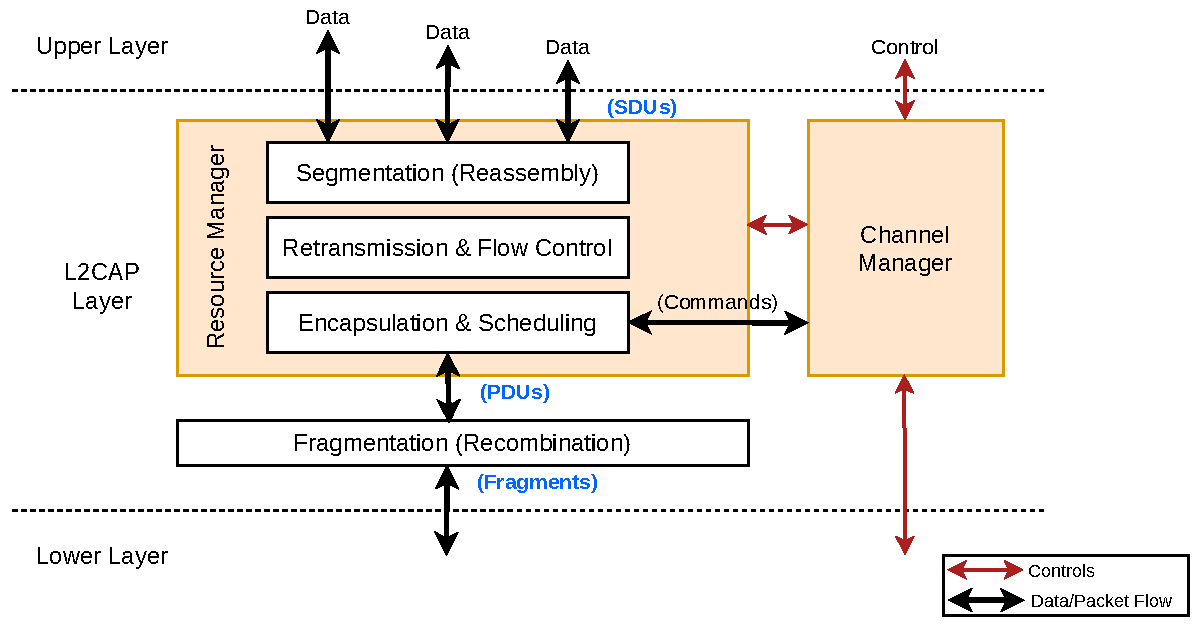
\includegraphics[width=0.9\textwidth]{graphics/l2cap_architektur.pdf}
    \caption[Architektur des L2CAP Layers]{Architektur des L2CAP Layers \cite{BtSpec4.0_1391}}
    \label{fig: l2cap architektur}
\end{figure}
% QUELLE l2cap layer resource manager channel manager spec 4.0 S. 1391

Der Channel Manager ist für die Verwaltung und Steuerung der L2CAP Channels zuständig. Das umfasst die auf L2CAP bezogene Signalübertragung intern, Peer"=to"=Peer, und zu höheren und niedrigeren Schichten \cite{BtSpec4.0_1390}. 
% QUELLE Spec. 4.0 S. 1390
Die Signale, die zwischen den zwei L2CAP"=Entitäten zweier verbundenen Geräte übertragen werden, sind Kommandos wie bspw. der LE Credit Based Connection Request und die entsprechende Response. Dafür wird ein separater L2CAP Channel mit der CID 0x0005 genutzt. Zudem betreibt der Channel Manager den L2CAP"=Zustandsautomaten, auf den hier nicht näher eingegangen werden soll.
\\\\
Da der L2CAP Layer nach unten mit dem Link Layer verknüpft ist (ggf. über das HCI), müssen die L2CAP PDUs dem Paketformat des Link Layers (bzw. dem HCI) gerecht werden. Dementsprechend werden die L2CAP PDUs fragmentiert bzw. wieder zusammengesetzt. Die Maximal PDU Payload Size (MPS) bezeichnet die maximale Größe des Payload einer PDU in Byte, die eine L2CAP"=Entität verarbeiten kann.
% TODOOPT BILD + VERWEIS Spec 4.0 S. 1487, Mischung aus Figure 7.1 und 7.2, vereinfacht darstellen: L2CAP PDU -> HCI Paket -> Link Layer Paket
\\\\
Ein Datenaustausch zwischen L2CAP und dessen höhergelegenen Schichten / Protokollen erfolgt in der Form von Service Data Units (SDU), wobei deren Ursprung immer aus einer höheren Schicht stammt. Die Maximum Transmission Unit (MTU) bezeichnet die maximale Größe einer SDU in Byte, die die höhergelegene Schicht verarbeiten kann. Die Segmentierung (bzw. Zusammensetzung) dieser SDUs wird vom Resource Manager ausgeführt und ist für alle Modi außer dem Basic L2CAP Mode relevant. Wenn keine Segementierung angewandt wird, ist die MTU gleich der MPS \cite{BtSpec4.2_1727}. Falls ein L2CAP Channel in einem anderen Modus als dem Basic L2CAP Modus agiert, ist der Resource Manager auch für die erneute Übertragung von PDUs und Flusskontrolle zuständig. Außerdem plant der Resource Manager zu welchem Zeitpunkt L2CAP Channel PDUs versenden können, um den L2CAP Channels mit Quality"=of"=Service"=Optionen genügend Ressourcen bezüglich der Buffer des Controllers freizugeben. \cite{BtSpec4.2_185} \cite{BtSpec4.2_1725-1726}

\paragraph{Struktur eines Datenpakets} \mbox{} \vspace{0.2cm} \\
Es existieren verschiedene Arten von L2CAP"=Datenpaketen, die den gennanten Modi zugeordnet sind. Der Basic L2CAP Mode unterstützt verbindungsorientierte und verbindungslose L2CAP Channel, während die restlichen Modi nur verbindungsorientierte L2CAP Channels nutzen.
In Abb. \ref{fig: l2cap pdu basic} ist die Paketstruktur einer L2CAP PDU im Basic L2CAP Mode (verbindungsorientiert) dargestellt.

\begin{figure}[H]
    \centering
    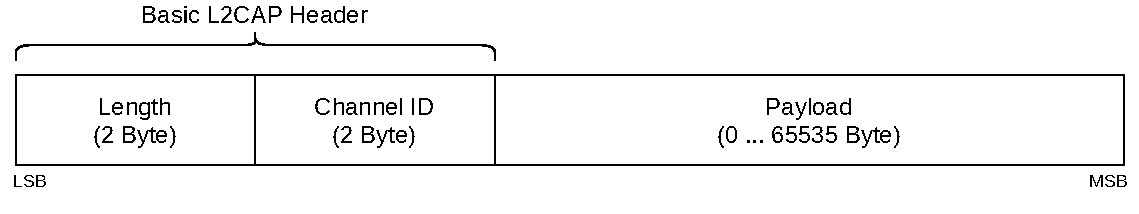
\includegraphics[width=0.9\textwidth]{graphics/l2cap_datenpaket.pdf}
    \caption[Struktur einer L2CAP PDU (Basic L2CAP Mode)]{Struktur einer L2CAP PDU (Basic L2CAP Mode) \cite{BtSpec4.2_fig_1737}}
    \label{fig: l2cap pdu basic}
\end{figure}
% QUELLE Spec. 4.2 S. 1737 Figure 3.1

LSB steht für Least Significant Bit, also das Bit mit niedrigstem Stellenwert, und MSB für Most Significant Bit, also das Bit mit höchstem Stellenwert. Das Längenfeld beschreibt die Länge des Payload, der eine maximale Länge von 65535 Byte besitzt.
\\\\
Abb. \ref{fig: l2cap pdu credit} zeigt die Paketstruktur einer L2CAP PDU im LE Credit Based Flow Control Mode.

\begin{figure}
    \centering
    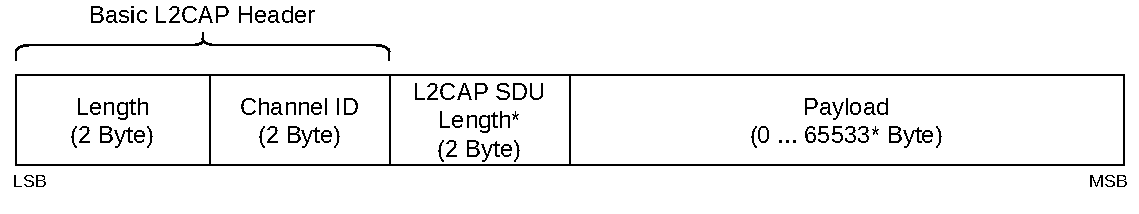
\includegraphics[width=0.9\textwidth]{graphics/l2cap_datenpaket_credit_based.pdf}
    \caption[Struktur einer L2CAP PDU (LE Credit Base Flow Control Mode)]{Struktur einer L2CAP PDU (LE Credit Base Flow Control Mode); *nur in erster PDU einer SDU; \cite{BtSpec4.2_fig_1747}}
    \label{fig: l2cap pdu credit}
\end{figure}
% QUELLE Spec 4.2 S. 1747 Figure 3.6

Das SDU"=Längenfeld ist nur in der ersten PDU einer SDU enthalten, um die Gesamtlänge der SDU in Byte zu beschreiben. Dadurch kann die Länge des Payloads einer solchen ersten PDU nur maximal 65533 Byte betragen, da der Wert des Längenfelds des Basic L2CAP Header auch das SDU"=Längenfeld umfasst. Alle zur SDU zugehörigen folgenden PDUs enthalten das SDU"=Längenfeld nicht, wodurch deren maximale Payload"=Länge 65535 Byte beträgt.

Im LE Credit Based Flow Control Mode regulieren die beiden Endpunkte mithilfe von Credits wie viele PDUs der jeweilige Endpunkt empfangen kann. Sind keine Credits mehr für einen Endpunkt (Empfänger) vorhanden, kann der andere Endpunkt (Sender) keine PDUs mehr an den Empfänger übermitteln und muss warten bis der Empfänger ein Credit"=Signalpaket sendet, das neue Credits freigibt. \cite{BtSpec4.2_1780}

		\subsubsection{Generic Attribute Profile}
			Das Generic Attribute Profile (GATT) dient zur Kommunikation zwischen Client und Server. Es basiert auf dem Attribute Protocol (ATT), welches ausgehend vom Server Attribute bereitstellt, die von einem oder mehreren Clients "`entdeckt"' werden können. Ein Attribut besteht aus einem Typ, der anhand des Universal Unique Identifier (UUID) identifiziert wird, einem Attribute Handle, um auf das Attribut zuzugreifen, und einem Wert, der von Server und Client ausgelesen bzw. überschrieben werden kann. Zudem ist es möglich, für Attribute Berechtigungen festzulegen (bspw. nur Lesen, nicht Schreiben). \cite{BtSpec4.0_1835}
% QUELLE Spec 4.0 S. 1835 3.1 Introduction
\\\\
Entsprechend der S. \pageref{fig: host controller architektur} Abb. \ref{fig: host controller architektur} ordnet sich ATT über L2CAP in den Protokollstapel ein.
\\\\
Möchte ein Client einen Attributwert lesen bzw. schreiben, dann sendet er einen Read Request bzw. einen Write Request an den Server. Dieser reagiert, indem er bei einem Read Request das Attribut an den Client sendet bzw. bei einem Write Request den Attributwert entsprechend ändert und dem Client eine Bestätigung sendet. Im Fall, dass ausgehend vom Server ein Attribut geändert werden soll, sendet dieser eine Notification oder eine Indication an den Client. Im Gegensatz zur Notification bestätigt der Client eine empfangene Indication. \cite{BtSpec4.0_1854-1855} \cite{BtSpec4.0_1861-1863}
% QUELLE Spec 4.0 S. 1854 f. 3.4.4.3 Read Request und 3.4.4.4 Read Response
% QUELLE Spec 4.0 S. 1861-1863 3.4.5.1 Write Request und 3.4.5.2 Write Response
\\\\
Die Daten werden in Form von Attribute Protocol PDUs (siehe Abb. \ref{fig: att pdu}) übertragen.

\begin{figure}[H]
    \centering
    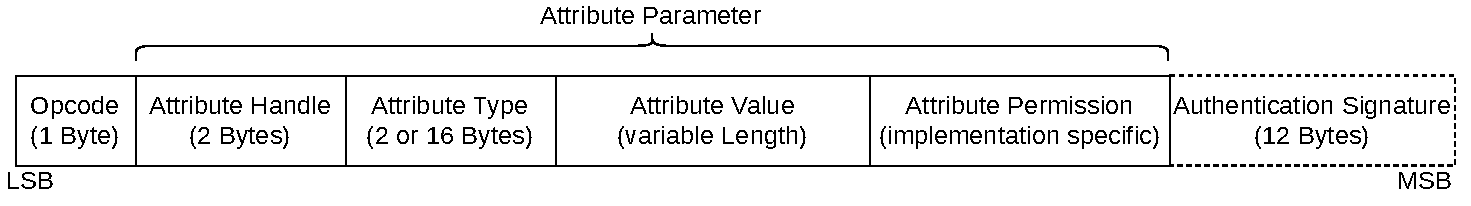
\includegraphics[width=0.9\textwidth]{graphics/att_pdu.pdf}
    \caption[(Generic) Attribute Protocol PDU]{(Generic) Attribute Protocol PDU; in Anlehnung an \cite{BtSpec4.0_fig_1888} und \cite{BtSpec4.0_fig_1889}}
    \label{fig: att pdu}
\end{figure}
% Quelle Spec 4.0 S. 1888 Figure 2.3 und S. 1889 Firgure 2.4

Der ein Byte lange Opcode sagt aus, ob die PDU entweder ein Request, eine Response, Notification, Indication oder Bestätigung ist, und enthält ein Flag für die Authentifizierung. Die Attributparameter unterteilen sich in zwei Byte für das Attribute Handle, zwei oder 16 Byte für den Attribute Type (die UUID), den Attributwert variabler Länge und die Attributberechtigungen, deren Länge von der Implementierung abhängig ist. Auf die Attributparameter folgt die 12 Byte lange Signatur für die Authentifizierung, falls gefordert. \cite{BtSpec4.0_1888-1889}
% QUELLE Spec 4.0 S. 1888 f.
\\\\

\begin{figure}{H}
    \centering
    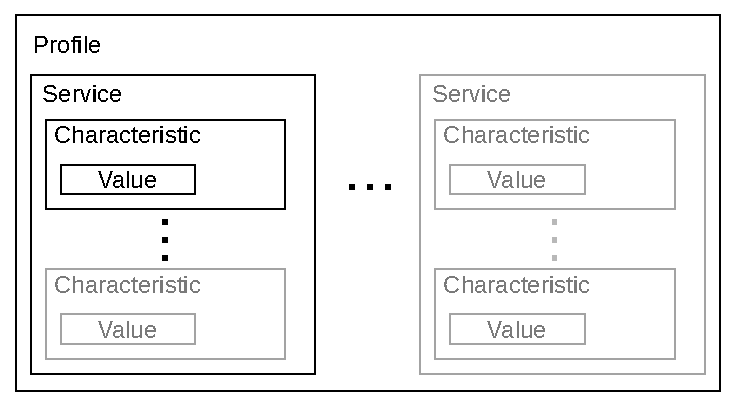
\includegraphics[width=0.9\textwidth]{graphics/gatt_hierarchie.pdf}
    \caption[]{\cite{BtSpec4.0_fig_1892}}
    \label{fig: gatt hierarchie}
\end{figure}
% Quelle Spec 4.0 S. 1892

GATT bildet eine Hierachie (siehe Abb. \ref{fig: gatt hierarchie}) bestehend aus den grundlegenden Elementen Profile, Service und Characteristic, die alle als Attribute definiert werden. An oberster Stelle befindet sich das Profile. Es enthält einen oder mehrere Services. Ein Service kann wiederum eine oder mehrere Characteristics enthalten, die sich aus Properties, einem Wert und Descriptors zusammensetzen.

		\subsubsection{Generic Access Profile}
			% TODO
Modes

Das Generic Access Profile (GAP) definiert verschiedene Rollen und Modi bzw. Prozeduren für Broadcasts und den Aufbau von Verbingungen.

Für LE existieren die vier Rollen: Broadcaster, Observer, Peripheral und Central. Ein Broadcaster ist aus Sicht des Link Layers (LL) ein Advertiser, da er verbindungslos Daten in Form von Advertising Events sendet. Der zugehörige Modus ist der Broadcast Mode. Diese Advertising Events können von Observern, die die Observation Procedure ausführen, empfangen werden, weswegen diese aus Sicht des LL als Scanner bezeichnet werden. Die Rolle Peripheral wird einem Gerät zugewiesen, wenn es den Aufbau eines LE Physical Link akzeptiert. Dabei nimmt es in Bezug auf den Link Layer die Rolle des Slave ein. Die Rolle Central wird einem Gerät zugewiesen, wenn dieses den Aufbau einer physischen Verbindung einleitet. Dabei nimmt es in Bezug auf den Link Layer die Rolle des Master ein. Ein Gerät kann mehrere Rollen zur selben Zeit einnehmen.
% TODO QUELLE Spec 4.0 S. 1638 f. 2.2.2 Roles when Operating over an LE Physical Channel
% TODO QUELLE Spec 4.0 S. 1695 f. 9.9.1 und 9.9.2

Jedes Gerät befindet sich entweder im Non-discoverable Mode, in dem es nicht von anderen Geräten entdeckt werden kann, oder im General Discoverable Mode bzw. im Limited Discoverable Mode, in denen es entdeckbar ist. Im Letzteren ist ein Gerät nur für eine bestimmte Dauer entdeckbar. Geräte, die andere Geräte entdecken sollen, müssen die General Discovery Procedure bzw. Limited Discovery Procedure ausführen.
% TODO QUELLE Spec 4.0 S. 1697 9.2 Discovery Modes And Procedures

Um Verbindungen und deren Aufbau zu steuern, gibt es mehrere Modi und Prozeduren, von denen einige in der Tabelle X zusammengefasst werden.
% TODO TABELLE VERWEIS

\begin{table}
    \begin{tabularx}{\textwidth}{|p{4.5cm}|X|}
    \hline
    \textbf{Modus/Prozedur} & \textbf{Beschreibung} \\
    \hline
    Non-connectable Mode & keine Verbindungen akzeptieren \\
    \hline
    Directed Connectable Mode & nur Verbindungen von bekannten Peer-Geräten akzeptieren, die die Auto oder General Connection Establishment Procedure ausführen \\
    \hline
    Undirected Connectable Mode & nur Verbindungen von Geräten akzeptieren, die die Auto oder General Connection Establishment Procedure ausführen \\
    \hline
    Auto Connection Establishment Procedure & Aufbau von Verbindungen zu Geräten, die in einem Connectable Mode sind und deren Adresse auf der Whitelist eingetragen ist \\
    \hline
    General Connection Establishment Procedure & Aufbau von Verbindungen zu bekannten Peer-Geräten, die in einem Connectable Mode sind \\
    \hline
    Connection Parameter Update Procedure & Peripheral oder Central kann Link-Layer-Parameter einer Verbindung ändern \\
    \hline
    \end{tabularx}
    \caption{Modi und Prozeduren für Verbindungen (Generic Access Profile)}
\end{table}
% TODO QUELLE Spec 4.0 S. 1704 - 1718 9.3 Connection Modes and Procedures

Zusätzlich verfügt GAP über Sicherheitsaspekte, die in Sektion X behandelt werden.
% TODO SEKTION VERWEIS BLE Sicherheit

		\subsubsection{Security Manager Protocol}
			Der Security Manager (SM) bzw. das Security Manager Protocol (SMP) ist dafür zuständig eine sichere Verbindung zwischen zwei Geräten (Master und Slave) aufzubauen. Dies umfasst im Wesentlichen das Pairing, welches zur Authentifizierung und Generierung eines Schlüssels dient, und die Verteilung von Schlüsseln. Entsprechend der Abb. \ref{fig: smp in bt} lässt sich der Security Manager bzw. das SMP in die BLE-Architektur einordnen.

\begin{figure}[H]
    \centering
    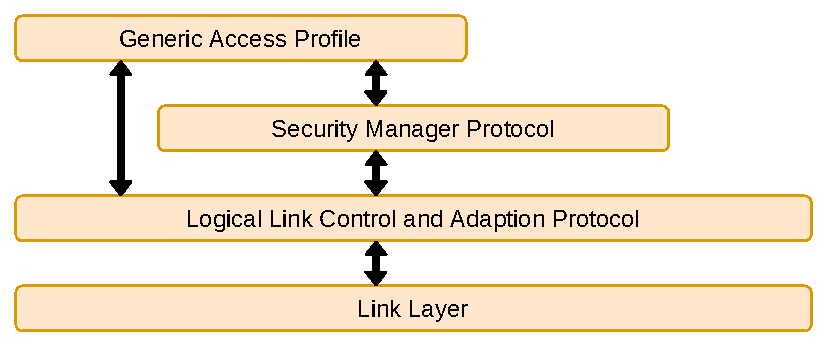
\includegraphics[width=0.8\textwidth]{graphics/smp_in_bt.pdf}
    \caption[Beziehungen des Security Managers zu anderen Host-Komponenten]{Beziehungen des Security Managers zu anderen Host-Komponenten; in Anlehnung an \cite{BtSpec4.0_fig_1958}}
    \label{fig: smp in bt}
\end{figure}
% QUELLE Spec 4.0 S. 1958

Um mit dem Link Layer zu interagieren, nutzt der SM einen L2CAP Channel mit einer festgelegten CID. Zudem kann er mit GAP direkt kommunizieren.
\\\\
Das Pairing lässt sich in drei Phasen aufteilen. Phase 1 und 2 dienen der Generierung eines Schlüssels, den beide Geräte zur Verschlüsselung und Authentifizierung im Link Layer nutzen. Dafür wird der Cipher Block Chaining - Message Authentication Code (CCM) Mode in Verbindung mit dem Advanced Encryption Standard (AES), genauer dem AES-128 Block Cipher, genutzt \cite{BtSpec4.0_2285}.
% QUELLE Spec. 4.0 S. 2285, 1 ENCRYPTION AND AUTHENTICATION OVERVIEW

\paragraph{Pairing: Phase 1} \mbox{} \vspace{0.2cm} \\
Die erste Phase ist der Pairing Feature Exchange, bei dem die beiden Geräte ihre für den Nutzer zugänglichen Ein- und Ausgabemöglichkeiten (IO Capabilities) austauschen. Die Tabellen \ref{tab: i caps geraet} und \ref{tab: o caps geraet} 
listen die entsprechenden Bezeichnungen dieser Möglichkeiten auf.
\\\\

\begin{table}[H]
    \begin{tabularx}{\textwidth}{|l|X|}
    \hline
    \textbf{Eingabemöglichkeit} & \textbf{Beschreibung} \\
    \hline
    Keine Eingabe & Gerät kann keine Eingaben entgegennehmen \\
    \hline
    Ja / Nein & Gerät kann zwei verschiedene Eingaben verarbeiten, die der Bedeutung Ja bzw. Nein zugewiesen werden können (bspw. zwei Tasten) \\
    \hline
    Tastatur & Eingabe der Ziffern 0 bis 9 möglich und die Möglichkeit Ja und Nein einzugeben \\
    \hline
    \end{tabularx}
    \caption[Eingabemöglichkeiten eines Gerätes]{Eingabemöglichkeiten eines Gerätes \cite{BtSpec4.0_1965}}
    \label{tab: i caps geraet}
\end{table}

\begin{table}[H]
    \begin{tabularx}{\textwidth}{|l|X|}
    \hline
    \textbf{Ausgabemöglichkeiten} & \textbf{Beschreibung} \\
    \hline
    Keine Ausgabe & Gerät kann keine 6-stellige Dezimalzahl dem Nutzer anzeigen bzw. kommunizieren \\
    \hline
    Numerische Ausgabe & Gerät kann eine 6-stellige Dezimalzahl dem Nutzer anzeigen bzw. kommunizieren \\
    \hline
    \end{tabularx}
    \caption[Ausgabemöglichkeiten eines Gerätes]{Ausgabemöglichkeiten eines Gerätes \cite{BtSpec4.0_1965_b}}
    \label{tab: o caps geraet}
\end{table}
% QUELLE für Tabellen: Spec 4.0 S. 1965 Table 2.1 und Table 2.2

Desweiteren tauschen die Geräte in der ersten Phase Informationen darüber aus, ob eine Authentifizierung zum Schutz vor einem Man-In-The-Middle-Angriff nötig ist (MITM Flag), und ob Daten für die Authentifizierung über die Pairing-Methode Out Of Band (OOB), d.h. mittels einer anderen Technologie (z.B. Near Field Communication), übertragen werden können (OOB Flag). Außerdem werden die minimalen und maximalen Größen für die Schlüssel ausgetauscht, die sich in 8 Bit großen Schritten zwischen 56 Bit (7 Byte) und 128 Bit (16 Byte) befinden. Dabei wird der kleinere Wert beider maximaler Größen übernommen. Falls die beiden Spannen sich nicht schneiden, wird das Pairing abgebrochen.

\paragraph{Pairing: Phase 2} \mbox{} \vspace{0.2cm} \\
Anhand der ausgetauschten Informationen aus der ersten Phase wird in der zweiten Phase entschieden, welche der folgenden Methoden zur Generierung des Short Term Key (STK) bzw. Long Term Key (LTK) zu verwenden ist:

\begin{itemize}
    \item{Numeric Comparison (für LE erst ab Bluetooth-Version 4.2)}
    \item{Just Works}
    \item{Out of Band (OOB)}
    \item{Passkey Entry}
\end{itemize}

Da das Pairing (speziell Phase 2) für LE in der Bluetooth-Version 4.0 funktionale Unterschiede zum Pairing für LE ab Version 4.2 aufweist, wird das Pairing für LE in Version 4.0 als \textbf{LE Legacy Pairing} und das Pairing für LE ab Version 4.2 als \textbf{LE Secure Connections Pairing} bezeichnet. Aus Sicht des Nutzers sind diese jedoch gleich und jede Bluetooth-Version, die LE unterstützt, unterstützt das LE Legacy Pairing. Im Gegensatz zum LE Secure Connections Pairing bietet LE Legacy Pairing für die Methoden Just Works und Passkey Entry keinen Schutz vor passivem Abhören während des Pairings, da LE Secure Connections Elliptic Curve Diffie-Hellman (ECDH) für den Schlüsselaustausch nutzt und LE Legacy Pairing nicht. \cite{BtSpec4.2_248}
% QUELLE Spec 4.2 S. 248 5.4.1 Association Models
\\\\
Haben beide Geräte OOB-Authentifizierungsdaten für das LE Legacy Pairing, wird unabhängig von der jeweiligen MITM-Flag die Methode OOB gewählt. In LE Secure Connections Pairing wird ebenso verfahren, nur dass hier nicht die OOB-Flag beider Geräte gesetzt sein müssen (aber können), da eine gesetzte OOB-Flag genügt. Ist die MITM-Flag beider Geräte nicht gesetzt, wird die Methode Just Works ausgeführt. Anderenfalls werden die Ein- und Ausgabemöglichkeiten der Geräte für die Wahl der Methode einbezogen entsprechend \cite{BtSpec4.2_tab_2302-2303}.
% Verweis TABELLE Spec 4.2 S. 2302 f., Table 2.8

\subparagraph{Pairing Methoden} \mbox{} \vspace{0.2cm} \\
Bei der \textbf{Numeric Comparison} wird dem Nutzer auf beiden Geräten jeweils eine zufällig generierte sechsstellige Dezimalzahl angezeigt. Diese muss der Nutzer vergleichen und im Falle der Übereinstimmung auf beiden Geräten bestätigen oder anderenfalls ablehnen. Somit kann der Nutzer unabhängig von der Namensgegebung der Geräte sicherstellen, die richtigen Geräte ausgewählt zu haben. Zudem bietet diese Methode Schutz vor MITM-Angriffen. Außenstehende, die Kenntnis über diese Zahl gewonnen haben, können laut \cite{BtSpec4.2_244-245} damit keinen Vorteil zur Entschlüsselung der zwischen den beiden Geräten ausgetauschten Daten erlangen, da die Zahl nicht als Eingabe zur Generierung eines Schlüssels verwendet wird.
% QUELLE VERWEIS Sepc 4.2 S. 244 f. 5.2.4.1 Numeric Comparison

\textbf{Just Works} basiert auf der Funktionsweise von Numeric Comparison mit dem Unterschied, dass hier dem Nutzer keine sechsstellige Dezimalzahl ausgegeben wird und er die Verbindung nur bestätigen muss. Dadurch bietet Just Works keinen Schutz vor MITM-Angriffen, aber einen Schutz gegen passives Abhören (außer für LE Legacy Pairing). \cite{BtSpec4.2_245}
% QUELLE Spec 4.2 S.245 5.2.4.2 Just Works

\textbf{Out of Band} ist die Nutzung einer anderen Technologie (z.B. Near Field Communication), um Geräte zu entdecken oder um kryptographische Informationen für den Pairing-Prozess auszutauschen. Dabei sollte die Technologie Schutz vor MITM-Angriffen bieten. \cite{BtSpec4.2_246}
% QUELLE Spec 4.2 S. 246 5.2.4.3 Out of Band

Die Methode \textbf{Passkey Entry} definiert, dass ein Gerät die zufällig generierte sechstellige Dezimalzahl ausgibt und der Nutzer diese auf dem anderen Gerät eingeben muss. Ein Schutz gegen MITM-Angriffe existiert, da diese nur mit einer Wahrscheinlichtkeit von 0,000001 für jede Durchführung der Methode möglich sind. Schutz gegen passives Abhören bietet Passkey Entry nur in LE Secure Connections Pairing und nicht in LE Legacy Pairing. \cite{BtSpec4.2_246-247} \cite{BtSpec4.2_2304}
% QUELLE Spec 4.2 S. 246 f. 5.2.4.4 Passkey Entry
% QUELLE Spec. 4.2 S. 2304 2.3.5.3 LE Legacy Pairing - Passkey Entry

\subparagraph{LE Legacy Pairing: Schlüssel und deren Generierung} \mbox{} \vspace{0.2cm} \\
Beim LE Legacy Pairing zweier Geräte generieren beide einen 128 Bit langen Temporary Key (TK), der bei der Authentifizierung genutzt wird, um den STK zu generieren und die Verbindung zu verschlüsseln. In Just Works wird der TK auf null gesetzt. Bei der Methode Passkey Entry ist der TK die besagte zufällig generierte sechstellige Dezimalzahl, die bereits mit 20 Bit dargestellt werden kann, weswegen die restlichen Bit des TK auf null gesetzt werden müssen. Dagegen kann bei OOB auf diese Einschränkung verzichtet werden, wodurch der TK wahrhaftig eine Länge von 128 Bit besitzt.

Das Gerät, welches das Pairing einleitet (Master), generiert eine zufällige 128 Bit große Nummer \textit{Mrand} und ermittelt den 128 Bit großen Bestätigungswert \textit{Mconfirm} mit der Confirm Value Generation Function c1 \cite{BtSpec4.2_2288}. 
% QUELLE Spec. 4.2 S. 2288 2.2.3 Confirm value generation function c1 for LE Legacy Pairing
Zur Berechnung von \textit{Mconfirm} erhält die Funktion c1 folgende Eingabewerte entsprechend Gl. \ref{eq: mconfirm} \cite{BtSpec4.2_2305-2306}.

\begin{equation}
\begin{split}
    \text{Mconfirm} = \text{c1}(& \text{TK, Mrand,} \\
    & \text{Pairing Request Command, Pairing Response Command,} \\
    & \text{Adresstyp des Masters, Adresse des Masters,} \\
    & \text{Adresstyp des Slaves, Adresse des Slaves}) \\
\end{split}
    \label{eq: mconfirm}
\end{equation}

Ebenso führt das antwortende Gerät (Slave) diese Schritte durch, wobei \textit{Mrand} als \textit{Srand} bezeichnet wird und \textit{Mconfirm} als \textit{Sconfirm}. Die Eingabewerte der Funktion c1 zur Berechnung von \textit{Sconfirm}sind demnach analog zu denen von \textit{Mconfirm}. Danach findet entsprechend Abb. \ref{fig: austausch vor stk generierung} folgender Austausch statt.

\begin{figure}[H]
    \centering
    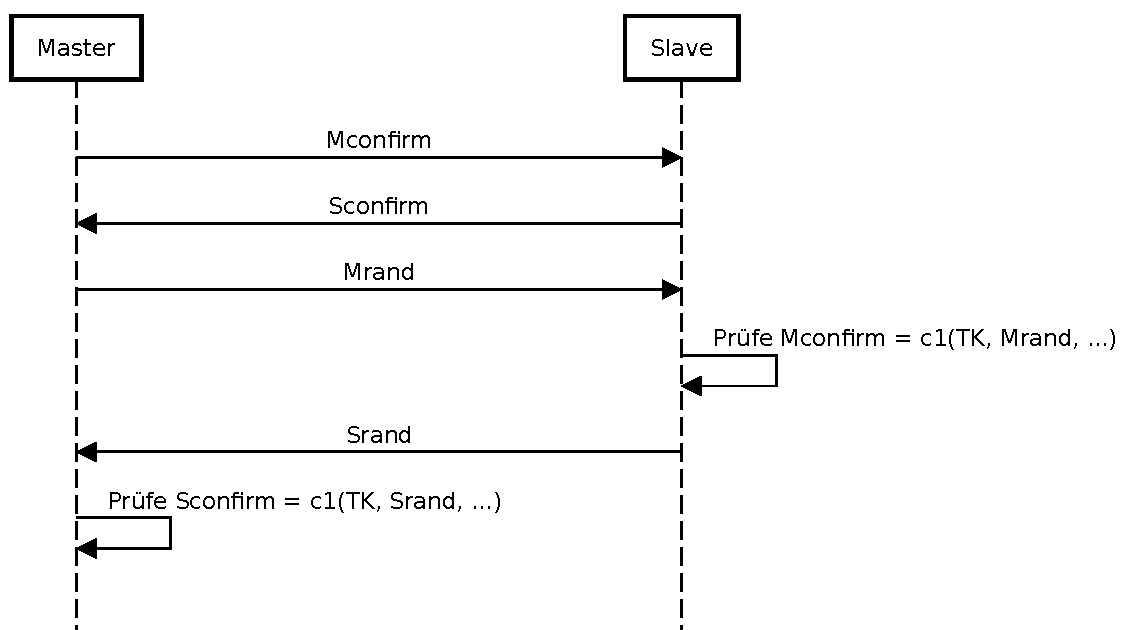
\includegraphics[width=0.9\textwidth]{graphics/austausch_vor_stk_generierung.pdf}
    \caption[Austausch von \textit{Mconfirm}, \textit{Sconfirm}, \textit{Mrand} und \textit{Srand} zwischen Master und Slave]{Austausch von \textit{Mconfirm}, \textit{Sconfirm}, \textit{Mrand} und \textit{Srand} zwischen Master und Slave \cite{BtSpec4.2_2305-2306}}
    \label{fig: austausch vor stk generierung}
\end{figure}

Master und Slave tauschen \textit{Mconfirm} und \textit{Sconfirm} aus. Danach überträgt der Master \textit{Mrand}, damit der Slave \textit{Mconfirm} entsprechend Gl. \ref{eq: mconfirm} berechnen und so den empfangenen \textit{Mconfirm} verifizieren kann. Nach einer erfolgreichen Prüfung von \textit{Mconfirm} überträgt der Slave \textit{Srand}, damit der Master \textit{Sconfirm} analog zu Gl. \ref{eq: mconfirm} berechnen und somit den empfangenen \textit{Sconfirm} verifizieren kann. Wenn einer der Bestätigungswerte (\textit{Mconfirm}, \textit{Sconfirm}) nicht erfolgreich verifiziert wird, wird die Verbindung sofort beendet.
\\\\
Anschließend wird der STK mit der Funktion s1 \cite{BtSpec4.2_2290} 
% QUELLE verweis auf Spec 4.2 S. 2290 2.2.4 Key generation function s1 for LE Legacy Pairing
entsprechend Gl \ref{eq: stk} \cite{BtSpec4.2_2305-2306} berechnet.

\begin{equation}
    \text{STK} = \text{s1}(\text{TK, Srand, Mrand})
    \label{eq: stk}
\end{equation}

Demnach kann bei der Methode Passkey Entry kein ausreichender Schutz gegen passives Abhören geboten werden, da der TK nur wenig mögliche Werte annehmen kann. Ist die vereinbarte Schlüsselgröße kleiner als 128 Bit, werden die überschüssigen Bit beginnend bei dem Bit mit dem höchsten Stellenwert auf null gesetzt. Der STK wird nun zur Verschlüsselung der Verbindung genutzt. \cite{BtSpec4.2_2305-2306}
% QUELLE Spec. 4.2 S. 2305 f. 2.3.5.5 LE Legacy Pairing Phase 2

\subparagraph{LE Secure Connections Pairing: Schlüssel und deren Generierung} \mbox{} \vspace{0.2cm} \\
Beim LE Secure Connections Pairing wird ein Long Term Key (LTK) erstellt. Zuvor erstellen beide Geräte jeweils ein ECDH-Schlüsselpaar (PK - Public Key, SK - Private Key) und tauschen ihre Public Keys aus. Danach berechnet jedes Gerät den Diffie-Hellman-Schlüssel aus seinem Private Key und dem Public Key des Anderen. Durch den Diffie-Hellman-Schlüssel kennen beide Parteien ein gemeinsames Geheimnis, mit dem sie den weiteren Datenaustausch zur Authentifizierung verschlüsseln können. Die Authentifizierung ist notwendig, da der ECDH-Schlüsselaustausch zwar resistent gegen passives Abhören ist, jedoch nicht gegen MITM-Angriffe. \cite{BtSpec4.2_2307}
% QUELLE Spec. 4.2 S. 2307 2.3.5.6.1 Public Key Exchange

Diese Authentifizierung wird mit den Pairing Methoden Numeric Comparison, Just Works, OOB und Passkey Entry ermöglicht. Jedoch unterscheiden diese sich aus funktionaler Sicht (nicht aus Nutzersicht) zum LE Legacy Pairing durch komplexere Verfahren. Letztendlich lässt sich für die vier Pairing-Methoden Folgendes zusammenfassen. Numeric Comparison signalisiert dem Nutzer mit einer Wahrscheinlichkeit von 0,999999 einen stattfindenden MITM-Angriff \cite{BtSpec4.2_2309}. 
% QUELLE Spec. 4.2 S. 2309, 2.3.5.6.2 Authentication Stage 1 – Just Works or Numeric Comparison
Just Works bietet keinen Schutz vor einem MITM-Angriff \cite{BtSpec4.2_245}. 
% QUELLE Spec. 4.2 S. 245, 5.2.4.2 Just Works
Ein MITM-Angriff während des Passkey Entry gelingt nur mit einer Wahrscheinlichkeit von 0,000001 \cite{BtSpec4.2_2311}. 
% QUELLE Spec. 4.2 S. 2311, 2.3.5.6.3 Authentication Stage 1 – Passkey Entry
Wie anfällig OOB für Angriffe ist hängt von der verwendeten OOB-Technologie ab \cite{BtSpec4.2_2312-2313}.
% QUELLE Spec. 4.2 S. 2312 f., 2.3.5.6.4 Authentication Stage 1 – Out of Band

Nach der Ausführung einer Pairing-Methode wird der LTK als Teilergebnis der Funktion f5 \cite{BtSpec4.2_2292-2293} 
% QUELLE Spec. 4.2 S. 2292 f., 2.2.7 LE Secure Connections Key Generation Function f5
mit den Eingabewerten Diffie-Hellman-Key, ein Nonce des Masters, ein Nonce des Slaves und der Adresse des Masters und Slaves ermittelt \cite{BtSpec4.2_2314}.
% QUELLE Spec. 4.2 S. 2314, 2.3.5.6.5 Authentication Stage 2 and Long Term Key Calculation

\paragraph{Pairing: Phase 3} \mbox{} \vspace{0.2cm} \\
Wurde der STK bzw. LTK generiert, wird dieser genutzt, um die Verbindung zu verschlüsseln. Nun können in der dritten Phase transportspezifische Schlüssel ausgetauscht werden. Z.B. wird der Identity Resolving Key (IRK) zur Generierung und Auflösung von zufälligen Adressen verwendet und der Connection Signature Resolving Key (CSRK) zur Signatur von Daten und Überprüfung von Signaturen.

% Für Numeric Comparison und Just Works wird entsprechend Abb. X fortgefahren.
% % TODO BILD VERWEIS

% \begin{figure}[hbt!]
%     \centering
%     \inlcudegraphics[width=0.5\linewidth]{graphics/LE_Secure_Connections_Pairing_Numeric_Comparison_Just_Works.svg}
%     \caption{}
% \end{figure}

% Der zu Beginn zufällig generierte Nonce (N\textunderscore a bzw. N\textunderscore b) mit einer Länge von 128 Bit wird für jeden Durchlauf neu erzeugt und schützt vor Replay-Angriffen. Für die Berechnung der Bestätigung C\textunderscore b wird die Einwegfunktion f4 [X] genutzt. 
% % TODO QUELLE Spec. 4.2 S. 2291 2.2.6 LE Secure Connections Confirm Value Generation Function f4
% Mittels der Funktion g2 [X] 
% % TODO QUELLE Spec 4.2 S. 2295 2.2.9 LE Secure Connections Numeric Comparison Value Generation Function g2
% werden die Dezimalzahlen D\textunderscore a und D\textunderscore b berechnet. Darauf werden diese dem Nutzer auf den Geräten ausgegeben und dieser muss deren Gleichheit bestätigen. Wird anstatt Numeric Comparison die Methode Just Works ausgeführt, dann werden D\textunderscore a und D\textunderscore b nicht berechnet und folglich nicht dem Nutzer gezeigt. Sollte ein Fehler auftreten wird das Protokoll abgebrochen und kann neu gestartet werden.

% Beim vorherigen ECDH-Schlüsselaustausch, kann ein MITM-Angriff angewandt werden. Eine einfache Variante, die keine Informationen der beiden angegriffenen Geräte zwischen diesen austauscht sondern mit diesen jeweils separat die Methode Numeric Comparison durchführt, endet darin, dass dem angegriffenem Nutzer mit einer Wahrscheinlichkeit von 0,999999 auf dessen Geräten zwei verschiedene Dezimalzahlen angezeigt werden. Eine andere Variante wäre aus Sicht des Angreifenden den Verkehr bestehend aus der Bestätigung C\textunderscore b, dem Nonce N\textunderscore a und N\textunderscore b nur weiterzuleiten. Jedoch wird der Master bei der Überprüfung der Bestätigung C\textunderscore b feststellen, dass diese nicht mit seinem Public Key PK\textunderscore a erstellt wurde, was zum Abbruch führt.\\\\
% % TODO QUELLE Spec. 4.2 S. 2308 f. 2.3.5.6.2 Authentication Stage 1 – Just Works or Numeric Comparison
% Passkey Entry
% OOB

	\subsection{Verbindungsaufbau / Pairing}

	\subsection{Sicherheitslücken}

\newpage
\section{Grundlagen zu Transport Layer Security}

	\subsection{Zertifikate}

	\subsection{Algorithmen}

	\subsection{Protokoll}

	\subsection{Sicherheit}

\newpage
\section{Infrastruktur}

	\subsection{Ziel der Infrastruktur}
		\input{sections/infrastruktur/ziel.tex}

	\subsection{Topologie}

	\subsection{Transport}

	\subsection{Sicherheit}

	\subsection{Verbindungsaufbau}

\newpage
\section{Implementierung}

	\subsection{Ziel der Implementierung}

	\subsection{Topologie}

	\subsection{Hardware und Software}

	\subsection{Transport und Sicherheit}

	\subsection{Ausleihprozess}

		\subsubsection{Verbindungsaufbau}

		\subsubsection{Beenden des Ausleihprozesses}

\newpage
\section{Ausblick}

\newpage
\section{Zusammenfassung}

\newpage
\printbibliography[heading=bibintoc]

\end{document}